\documentclass{puzzlehunt}

\usepackage[final]{pdfpages}
\usepackage{amsmath,amssymb}
\usepackage{pgf,tikz}
\usetikzlibrary{arrows}

\usepackage{array}

\usepackage{environ}

\usepackage{chessfss}

\usepackage{multicol}
\usepackage{multirow}


% Contest name macros
\newcommand{\phEventName}{Mathematical Puzzle Programs}
\newcommand{\phEventAbbr}{Mathematical Puzzle Programs}


\title{\phEventName}
\author{Mathematical Puzzle Programs}
\date{\today}

% \phMarkDraft

\phSetSquareLogo{assets/mapp-square.pdf}
\phSetBannerLogo{assets/mapp-banner.pdf}

\begin{document}

\phChapterWorksheet{Getting on Top of Things}{Example Puzzle}

A friend passes you a note with the following strange image.

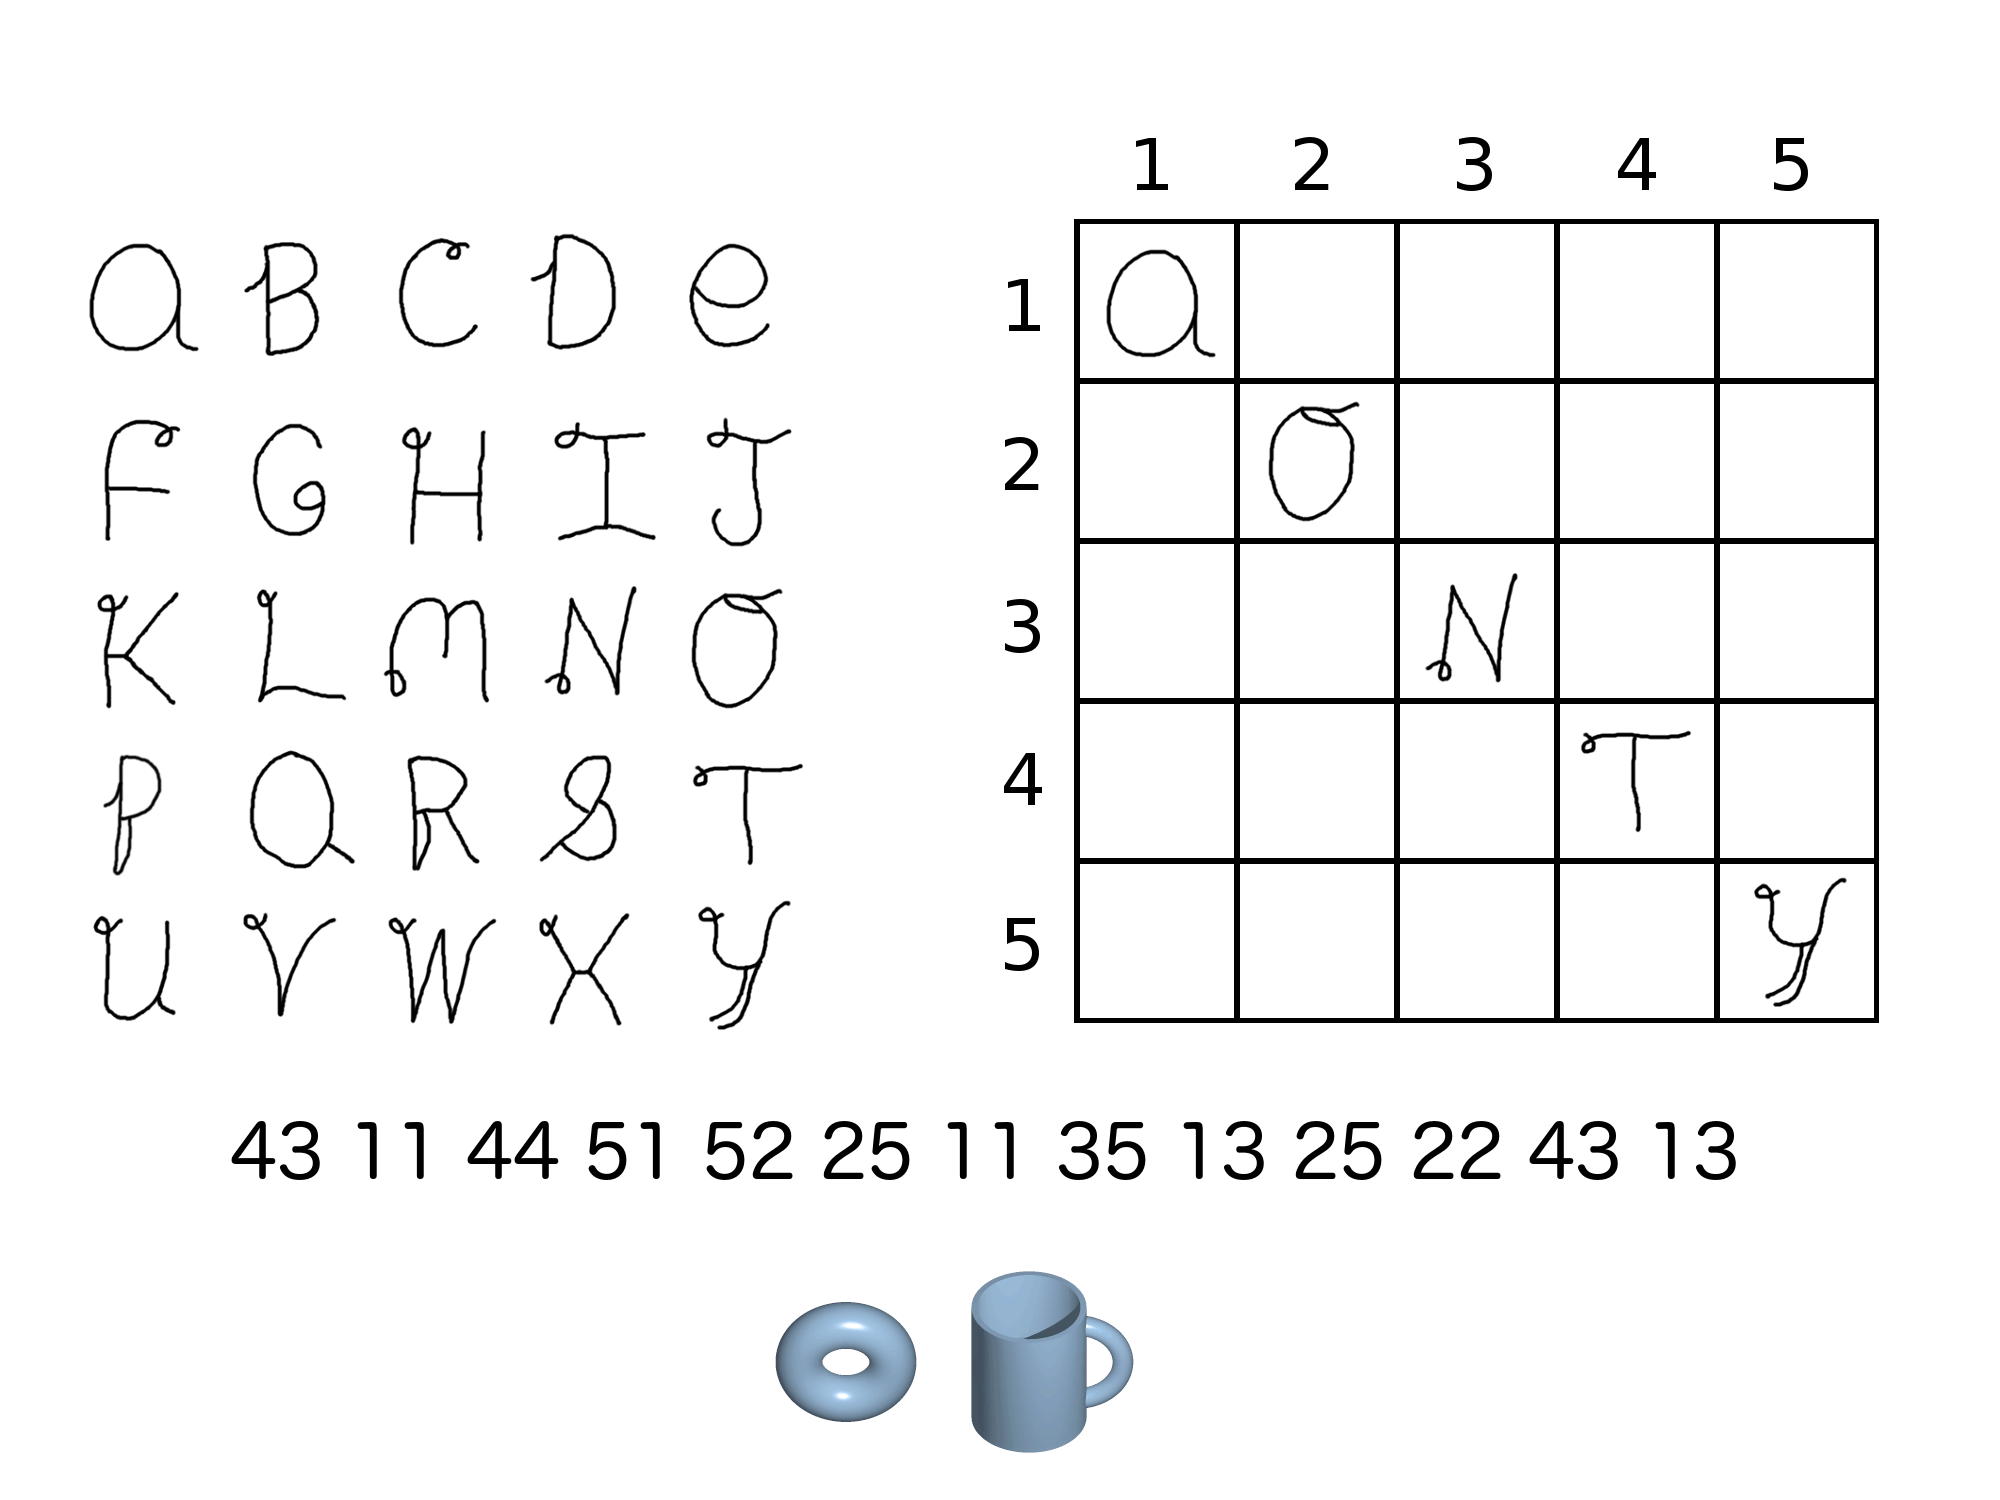
\includegraphics[width=0.9\linewidth]{assets/topology-puzzle.png}

She's recently been interested in \textbf{topology}, the study of structures
that can be morphed from one to another without cutting or tearing, such as
the donut and coffee cup shown in the image.

In each row of the above grid, fill in the other four letters that
are ``topologically equivalent'' to the given letter, in alphabetical
order. If you can do this correctly, each pair of numbers below the grid
can be decoded to a letter by using the rows/columns of the grid, spelling
a hidden message. Good luck!

\phChapter{About MaPP}

The mission of Mathematical Puzzle Programs (MaPP) is to organize quality events
which get students having fun by learning and using mathematics.

\begin{itemize}
\item \textbf{Math}\newline
Our mathematical content is pulled from various areas unrepresented in the
usual secondary curriculum,
such as design theory, game theory, or topology.

\item \textbf{Puzzles}\newline
We shredded the multiple choice tests, and instead designed several
mathematical puzzles which will
give your students a taste of real mathematical problem solving, and prepare
them for the types of questions asked in many job interviews.

\item \textbf{Team-Building}\newline
MaPP features a team-based competitions, emphasizing collaboration and
communication over individual work, as teamwork is crucial for success in both
industry and academia.

\item \textbf{FUN!}\newline
Many of the challenges can't be solved sitting down - players will find
themselves running around their
host campus to track down clues and uncover new puzzles to solve.
\end{itemize}

\vspace{2em}

  \phSection{Contact}

  \begin{itemize}
  \item Web: MaPPmath.org
  \item Twitter: @MaPPmath
  \item Email: info@mappmath.org
  \end{itemize}

\end{document}

%%% Local Variables:
%%% mode: latex
%%% TeX-master: t
%%% End:
